\chapter{Experimental Results from Corroded Rebar Specimens}
The results from the experimental program are summarized in this chapter and the implications for structural design are evaluated.

\section{Measurement of corrosion level}

\section{Tensions Tests}

As described in Chapter 3, the bars were loaded in tension using the universal testing machine (UTM). The data collected corresponded to the Force using the UTM and the Optotrack system was used to calculate the strain.

During the tests it was observed that the failure usually occurred close to the grips. This is due to the sudden change in the cross section and the imperfections on the rebars. The strains used in this study correspond to the strain gauges located adjacent to the fracture. The fracture of these tests were brittle in nature, the appearance of necking was not significantly observable. It is possible that necking occurred in a very localized manner. 

\fref{fig:TensionTestResults_StressStrain} show the stress-strain behavior for corrosion levels raging from 0 - 20\%. From this results, the yield strength, the uniform axial elongation, and the ultimate strength are obtained From this results it appears that the effective yield strength and the effective ultimate strength reduce as the corrosion level increases. In addition, the stress strain curves  results confirm that no necking significant necking was present, since were the after reaching the ultimate stress the bars suddenly drop  in strength. 

\begin{figure}[htbp]
	\centering
	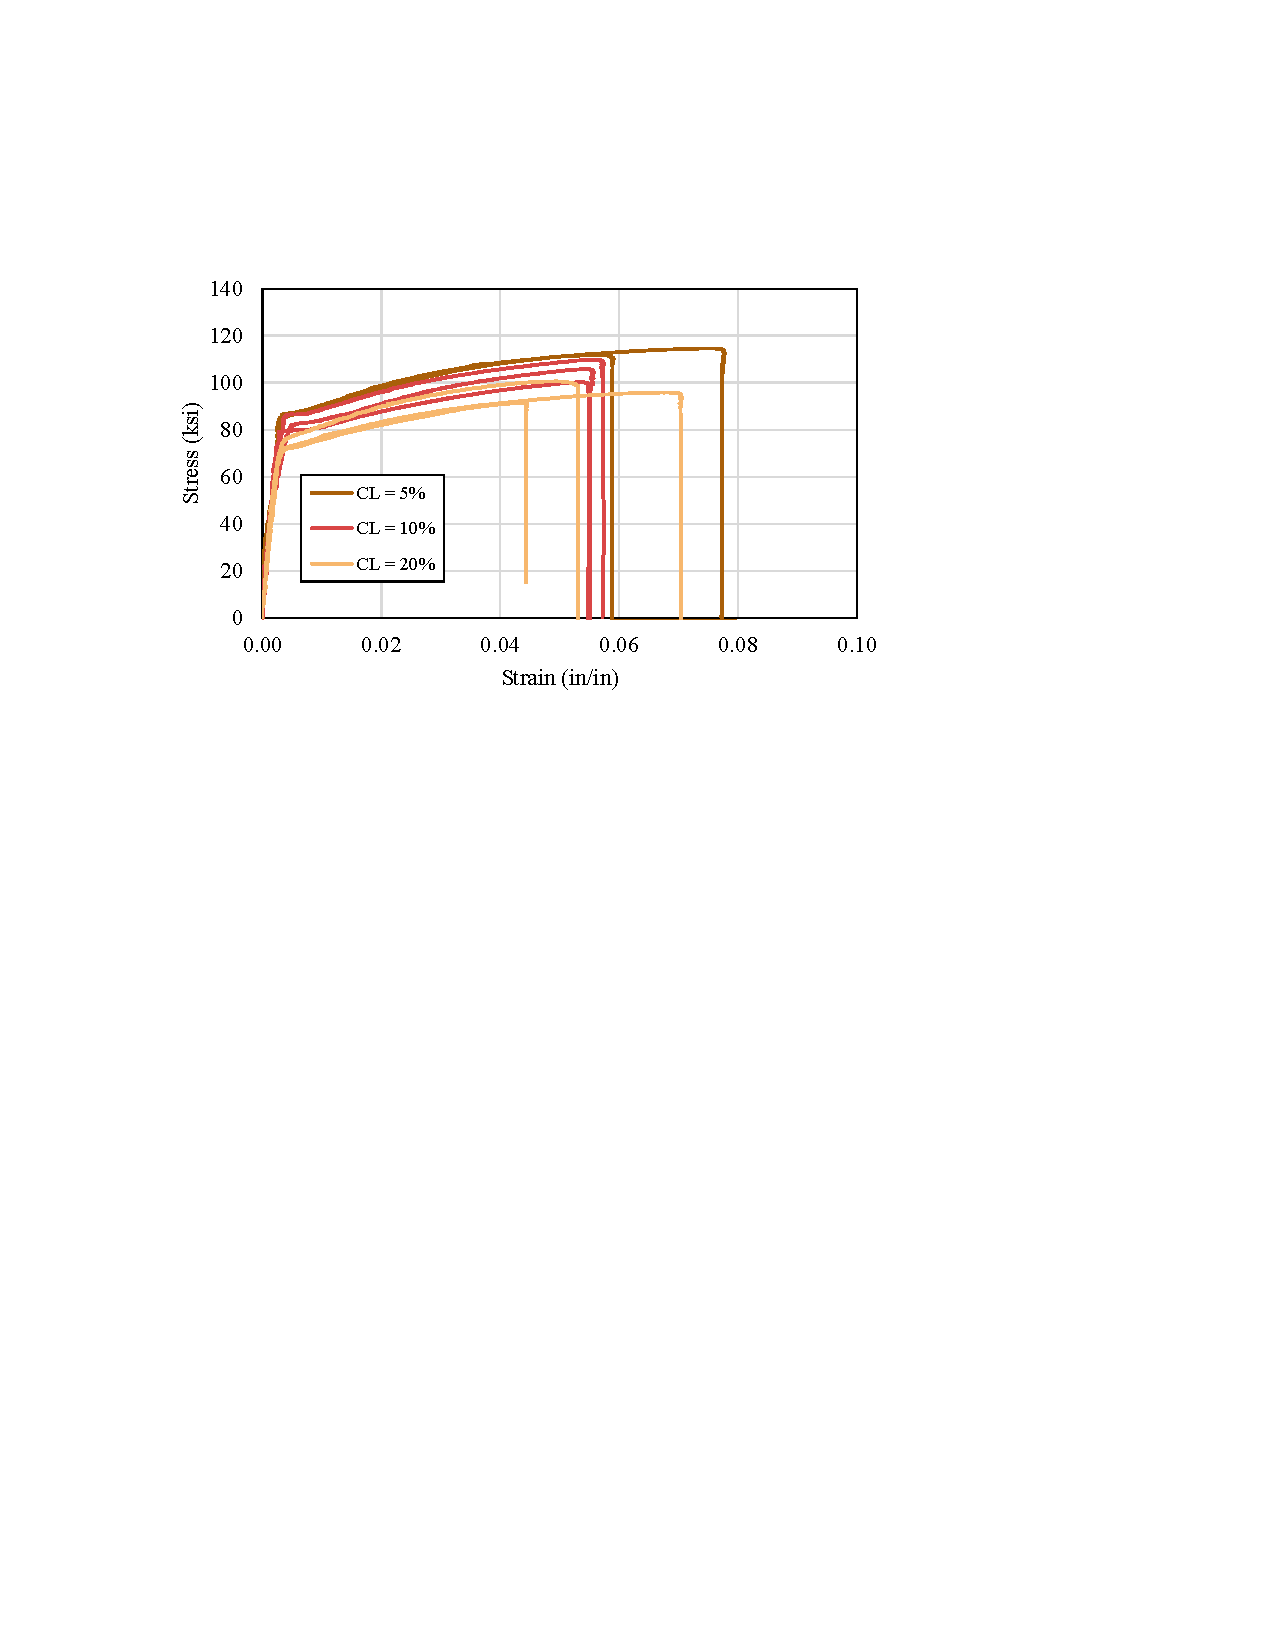
\includegraphics[width=0.7\textwidth]{VAC Thesis 2.0/Chapter-4/figs/TensionTest_results_1.pdf}
	\caption{Tension test results at different corrosion levels}
	\label{fig:TensionTestResults_StressStrain}
\end{figure}

\subsection{Yield strength as a function of corrosion}
\fref{fig:YieldStrength_vs_CL} shows the plot of the effective yield strength versus the corrosion level. The results show that there appears to be a linear relationship between them. This is congruent with other studies performed in other types of steel such as the study done by Du et al \cite{Du2005}. It has been studied that the apparent reduction in effective yield strength is due to points of concentrated reduction in the geometry of the rebars. Other studies \cite{Du2005}\cite{Barcley2018} and this study, show that if the imperfections due to the corrosion are removed, then the properties of the virgin metal remain unchanged. What is observed in tension tests conducted on corroded rebars is an effective property that considers the imperfections in the geometry of the rebar. 

The linear trend observed between the effective yield strength and the corrosion level can be expressed as:

\begin{equation}
    f_{y,CL} = f_{y,o}(1-0.0075CL)
    \label{eq.Calderon_Fy_vs_CL}
\end{equation}


\begin{figure}[htbp]
	\centering
	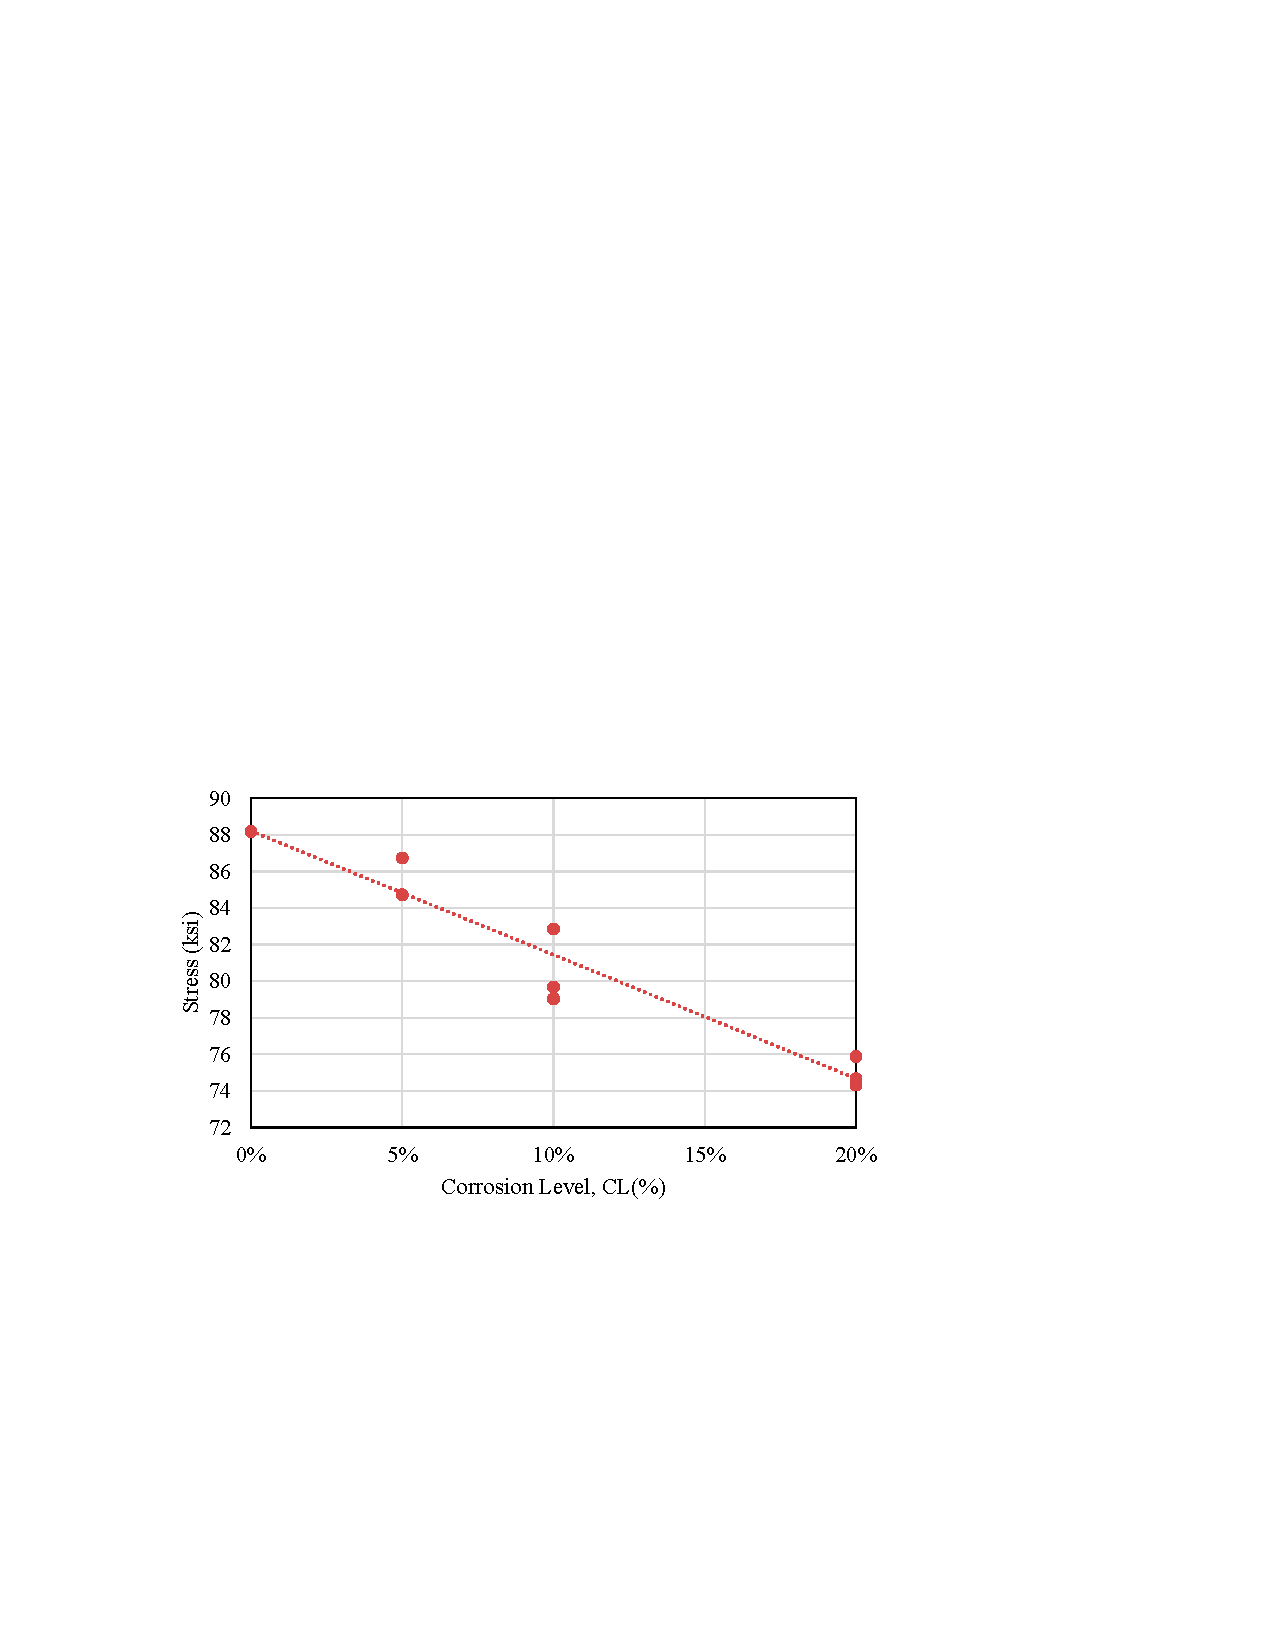
\includegraphics[width=0.7\textwidth]{VAC Thesis 2.0/Chapter-4/figs/TensionTest_results_2.pdf}
	\caption{Yield strength as a function of corrosion level}
	\label{fig:YieldStrength_vs_CL}
\end{figure}

The proposed equation is compared to the one proposed by Du et al \cite{Du2005}, replicated here as \ref{}. From \fref{fig:Calderon_vs_Du} we can observe that the existing model tends to over-predict the effective yield strength for Grade 80 steel. Therefore it is possible that there is correlation between corrosion level and the grade of the rebar, however the literature on corrosion for different grades of rebar is scarce. 

\begin{figure}[htbp]
	\centering
	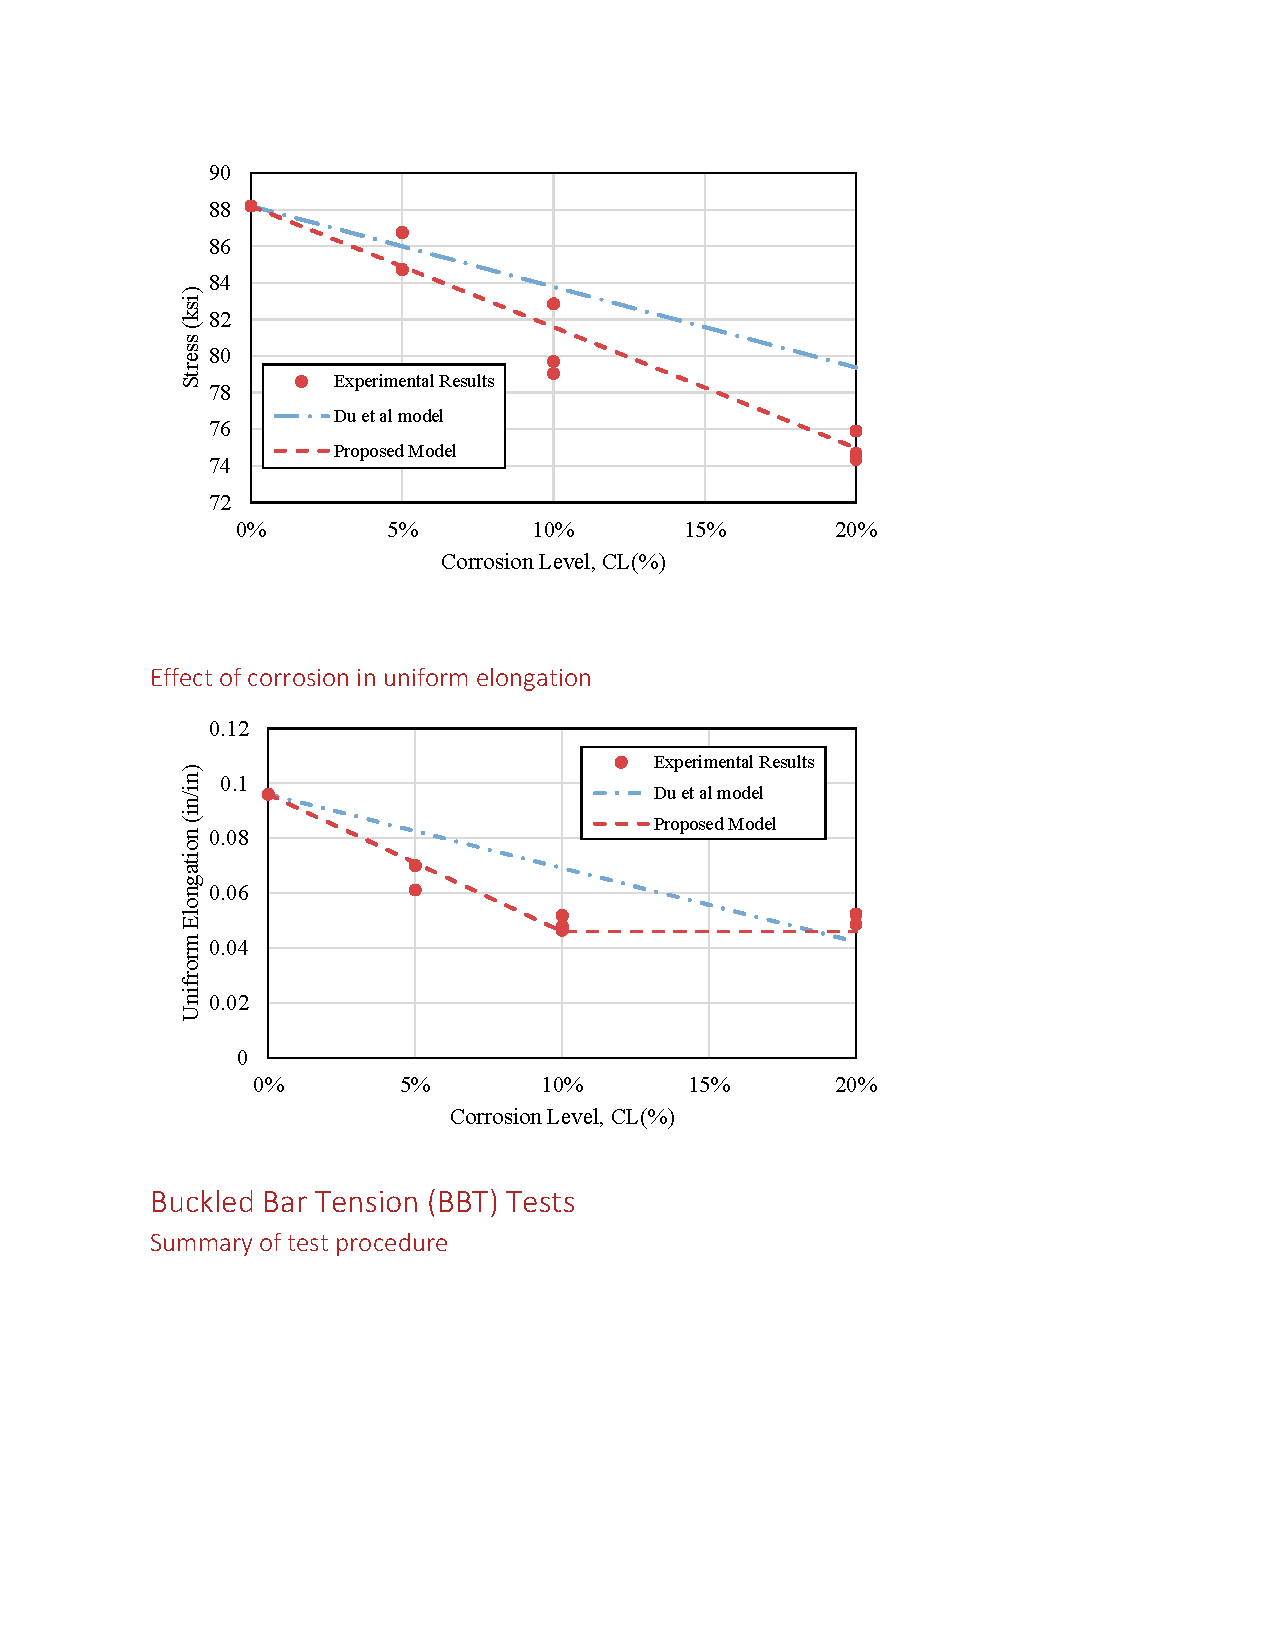
\includegraphics[width=0.7\textwidth]{VAC Thesis 2.0/Chapter-4/figs/TensionTest_results_3_proposedmodel.pdf}
	\caption{Yield strength as a function of corrosion level comparison of proposed model and Du et al model \cite{Du2005}}
	\label{fig:Calderon_vs_Du}
\end{figure}

\subsection{Effect of corrosion in uniform elongation}

Another insteresting result was observed on the uniform axial elongation property of the corroded rebars. As the rebar corrodes and develops more imperfections on the geometry of the rebar, it appears that the uniform axial elongation decreases.\fref{fig:UAE_vs_CL} shows this trend. However, after 10\% corrosion the uniform axial elongation remains constant. This results may point towards why as structure corrode the level of perceived ductility is reduced and thus triggers an earlier failure than that observed on pristine structures.

We propose the following model to predict the uniform axial elongation of corroded grade 80 rebars:

For corrosion level between 0\% - 10\%
\begin{equation}
    \varepsilon_{CL} = 0.05CL+\varepsilon_{o}
    \label{eq.Calderon_UAE_vs_CL}
\end{equation}

For corrosion level larger than 10\%

\begin{equation}
    \varepsilon_{CL} = 0.05CL+\varepsilon_{o}
    \label{eq.Calderon_UAE_vs_CL20}
\end{equation}

While equations \ref{eq.Calderon_Fy_vs_CL} - \ref{eq.Calderon_UAE_vs_CL20} are preliminary they provide an insight at the variations that different grades of rebar can have on the effective properties of corroded rebars.

\begin{figure}[htbp]
	\centering
	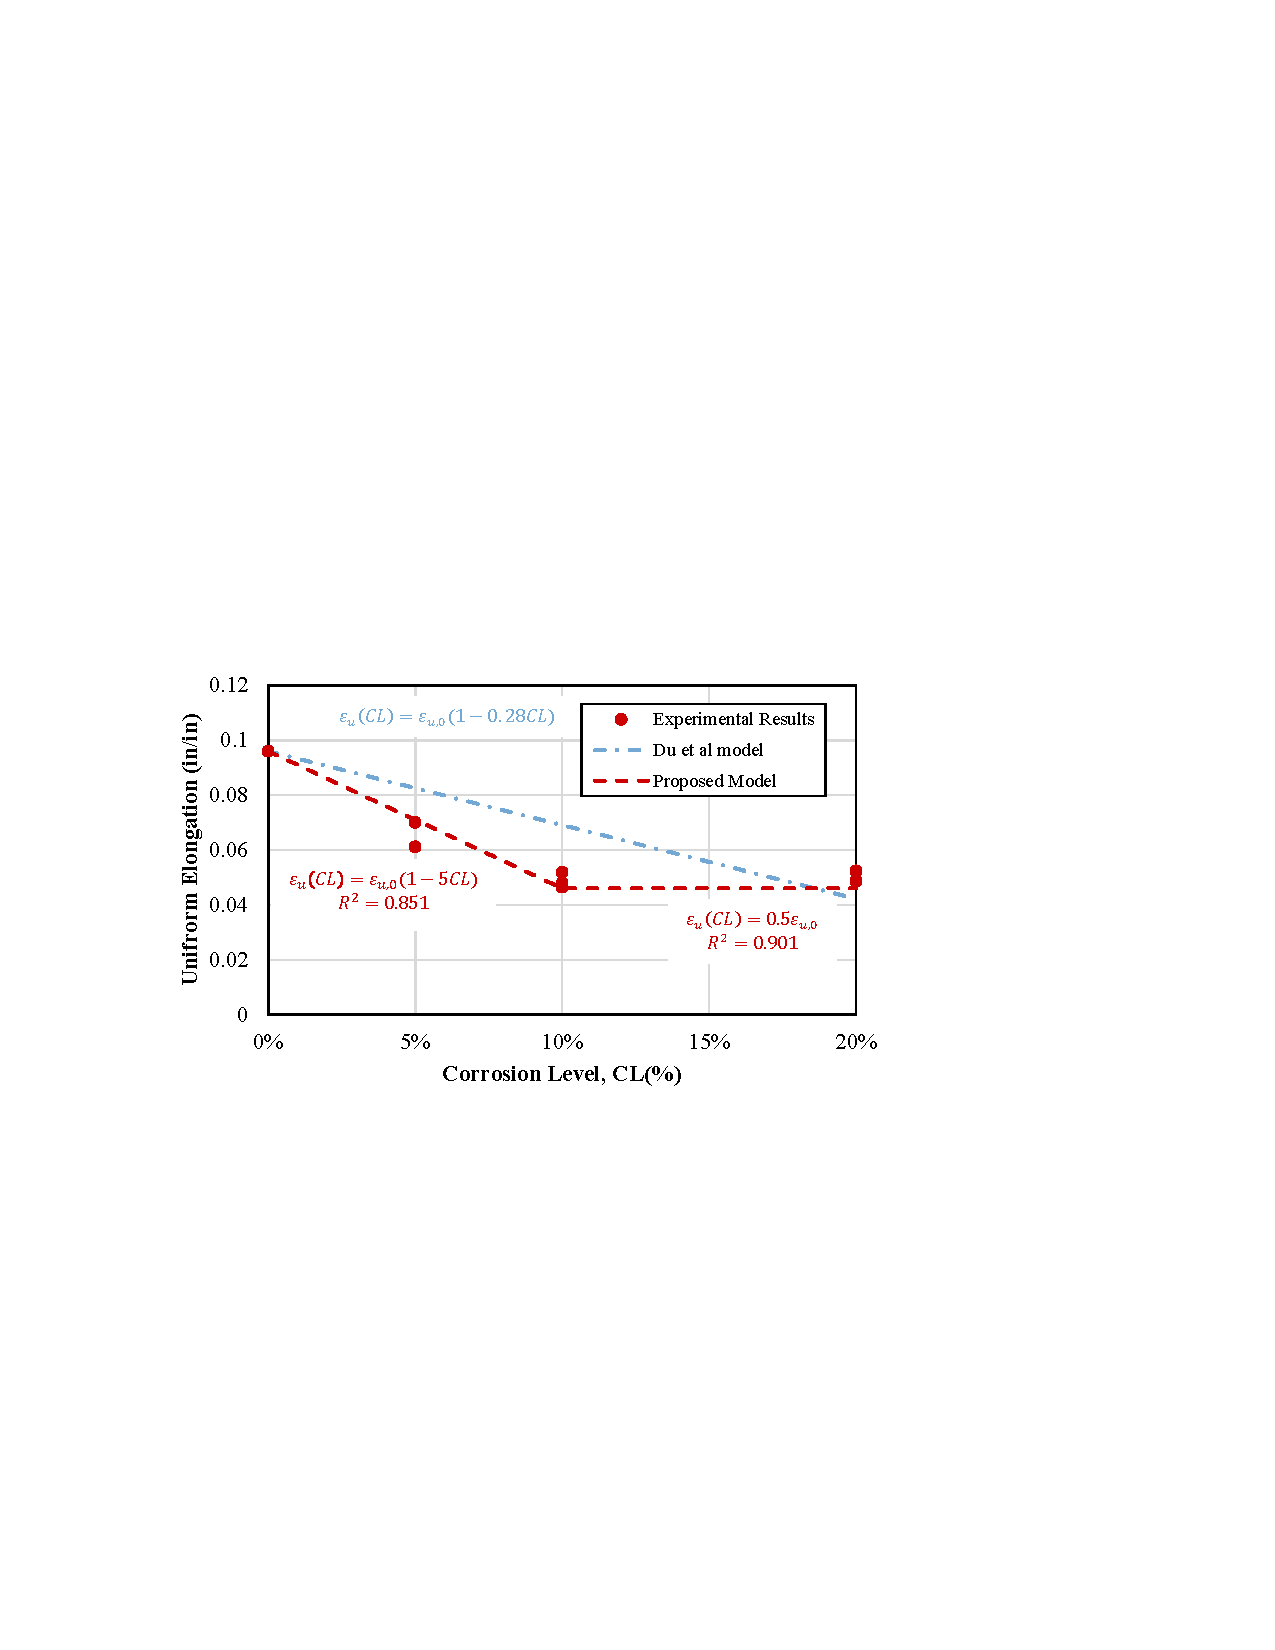
\includegraphics[width=0.7\textwidth]{VAC Thesis 2.0/Chapter-4/figs/TensionTest_results_4_proposedmodel.pdf}
	\caption{Uniform elongation as a function of the corrosion level comparison of proposed model and Du et al model \cite{Du2005}}
	\label{fig:UAE_vs_CL}
\end{figure}

\section{Buckled Bar Tension (BBT) Tests}

\begin{figure}[htbp]
	\centering
	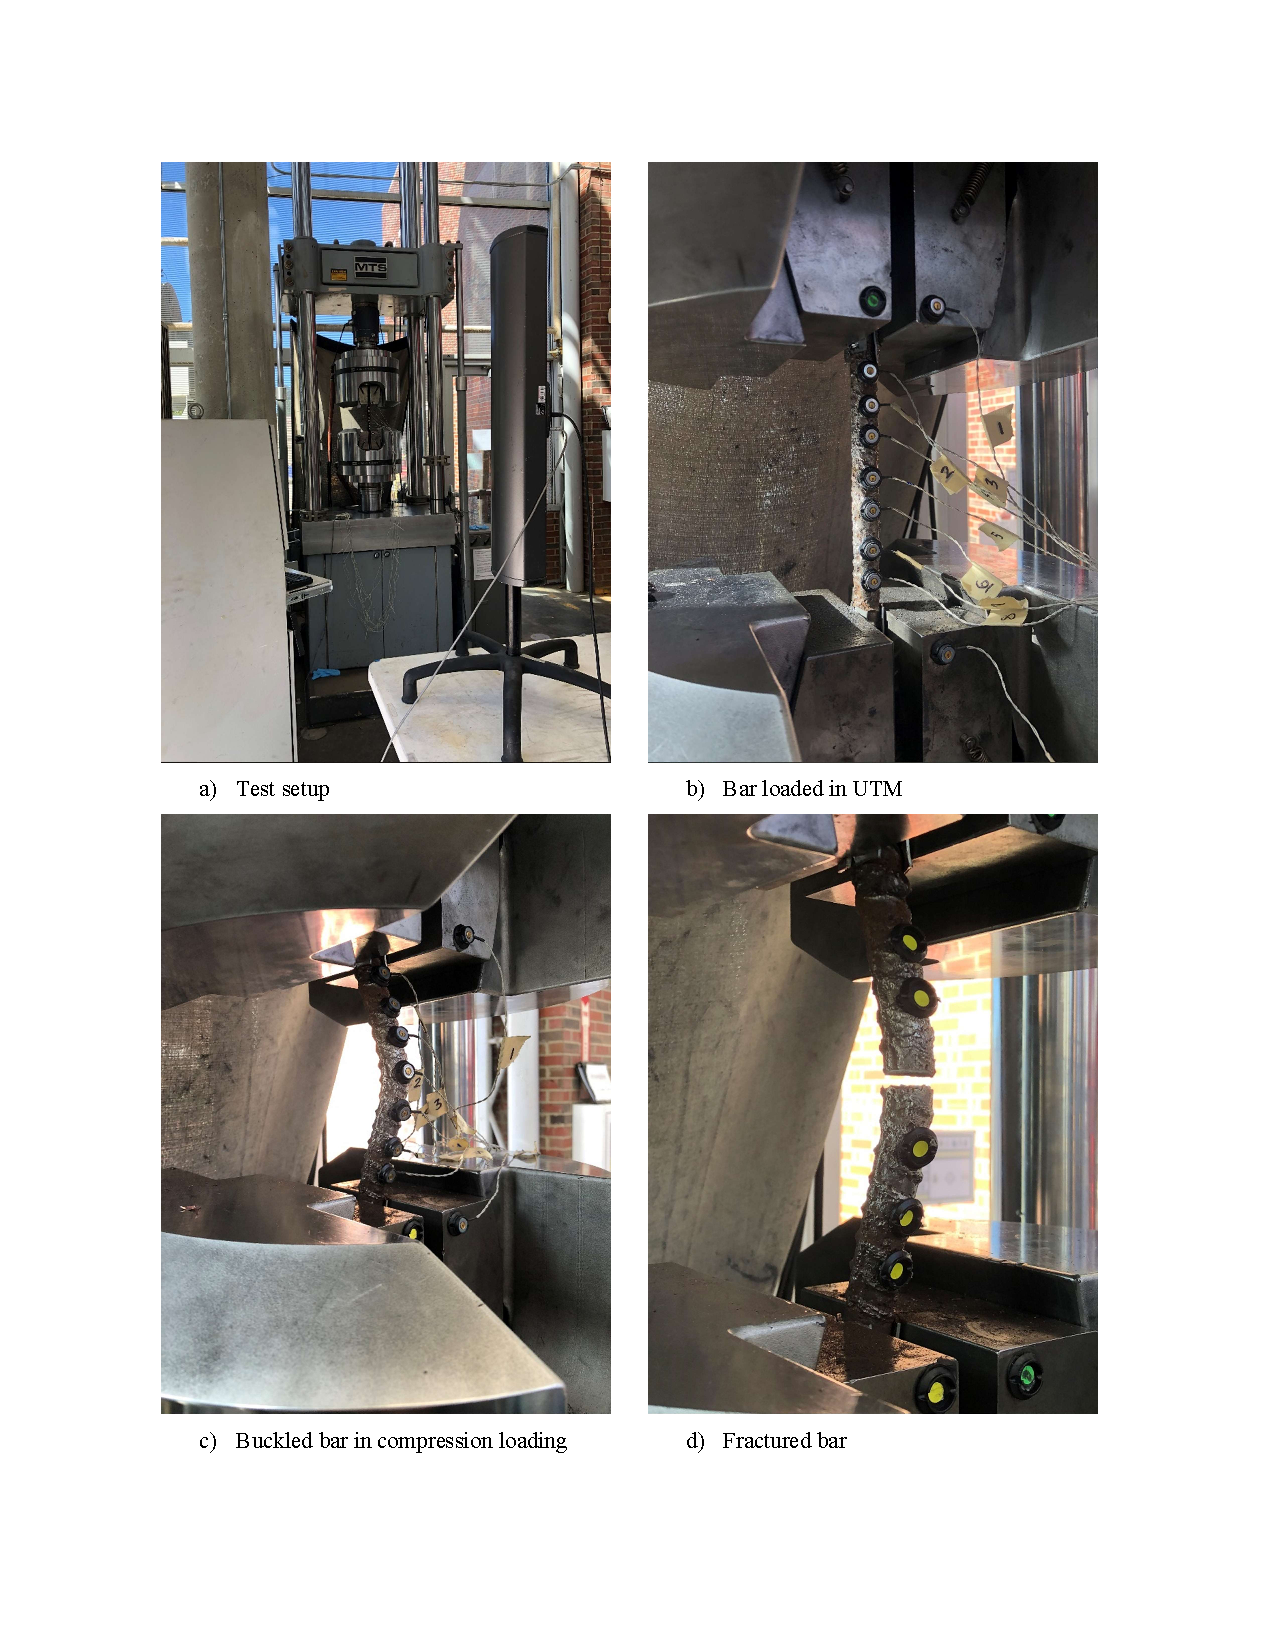
\includegraphics[width=0.7\textwidth]{VAC Thesis 2.0/Chapter-4/figs/BBT Procedure.pdf}
	\caption{General procedure of buckled bar tension (BBT) test}
	\label{fig:BBT_Test_Summary}
\end{figure}

\begin{figure}[htbp]
	\centering
	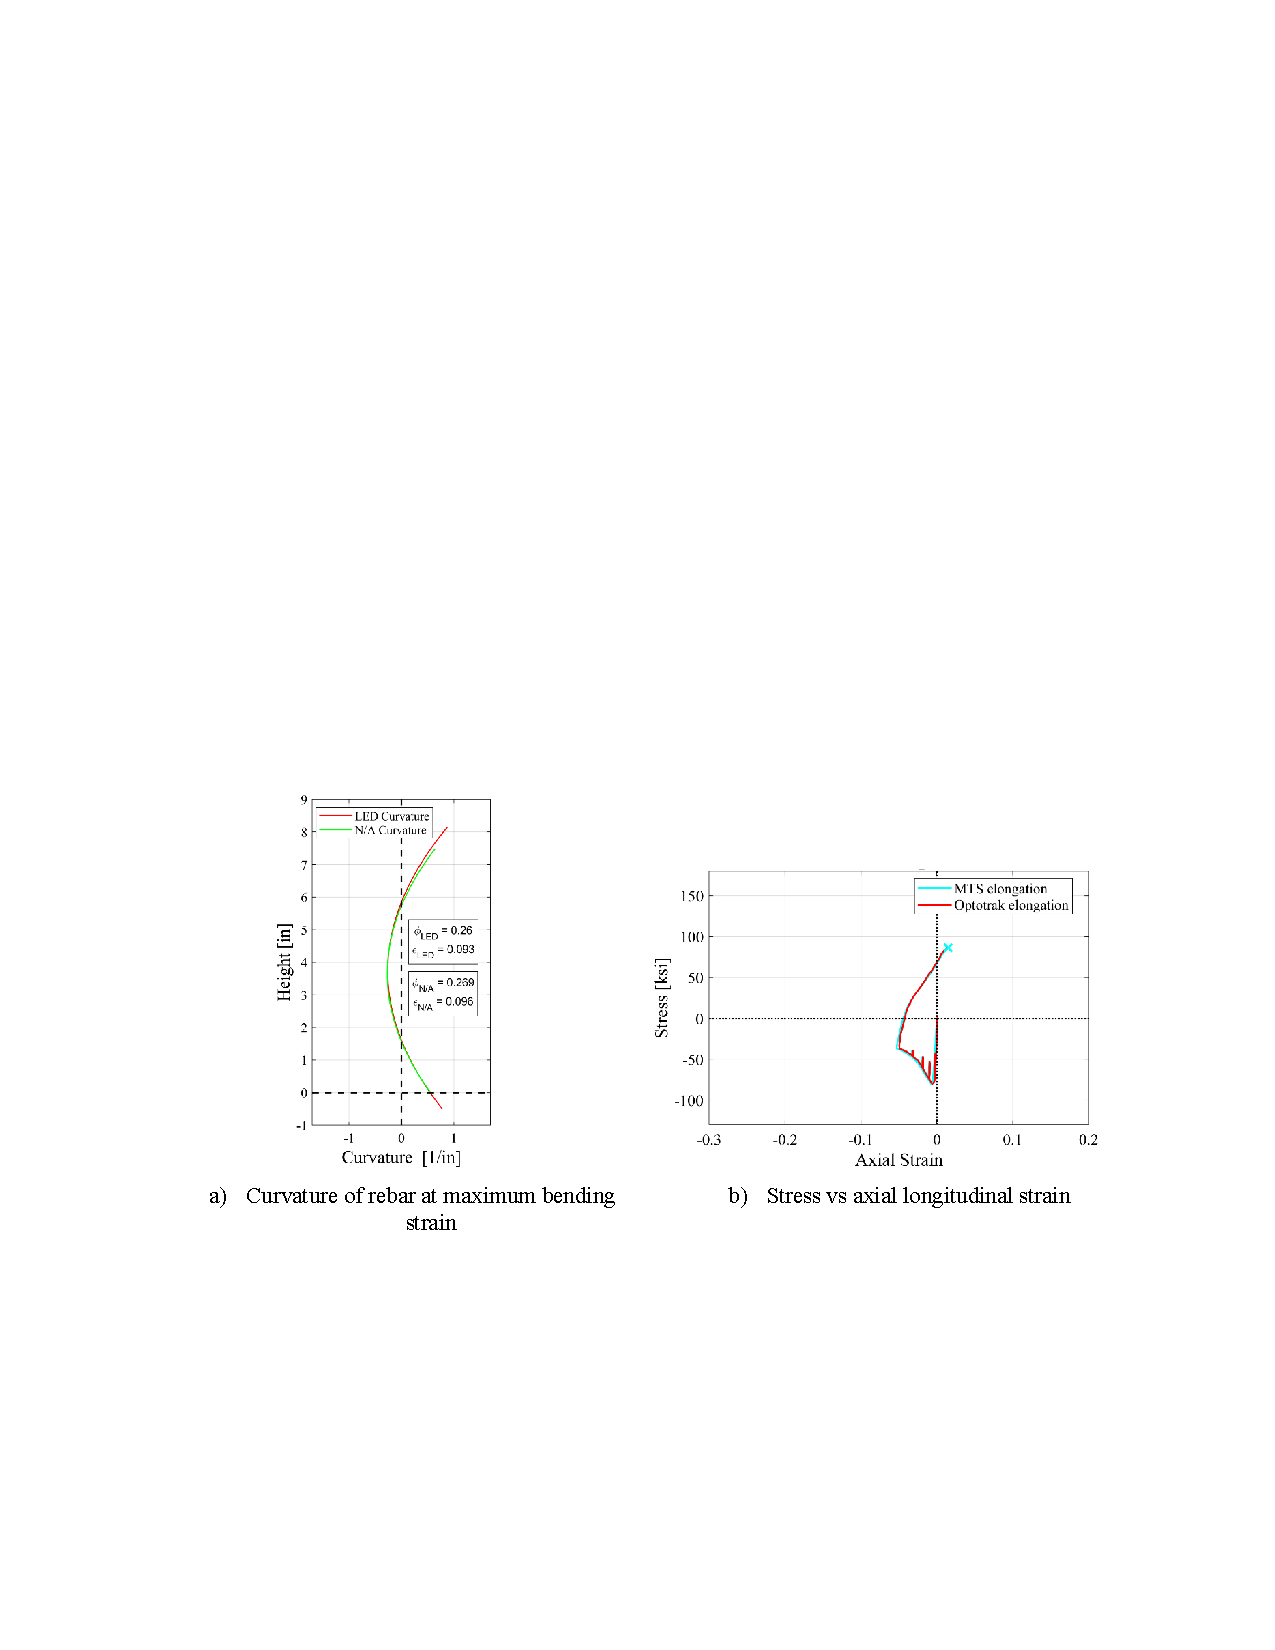
\includegraphics[width=1\textwidth]{VAC Thesis 2.0/Chapter-4/figs/BBT_curvature.pdf}
	\caption{Obtaining critical bending strain}
	\label{fig:bendingstrain}
\end{figure}

\subsection{Effect of corrosion in Critical Bending Strain}

\begin{figure}[htbp]
	\centering
	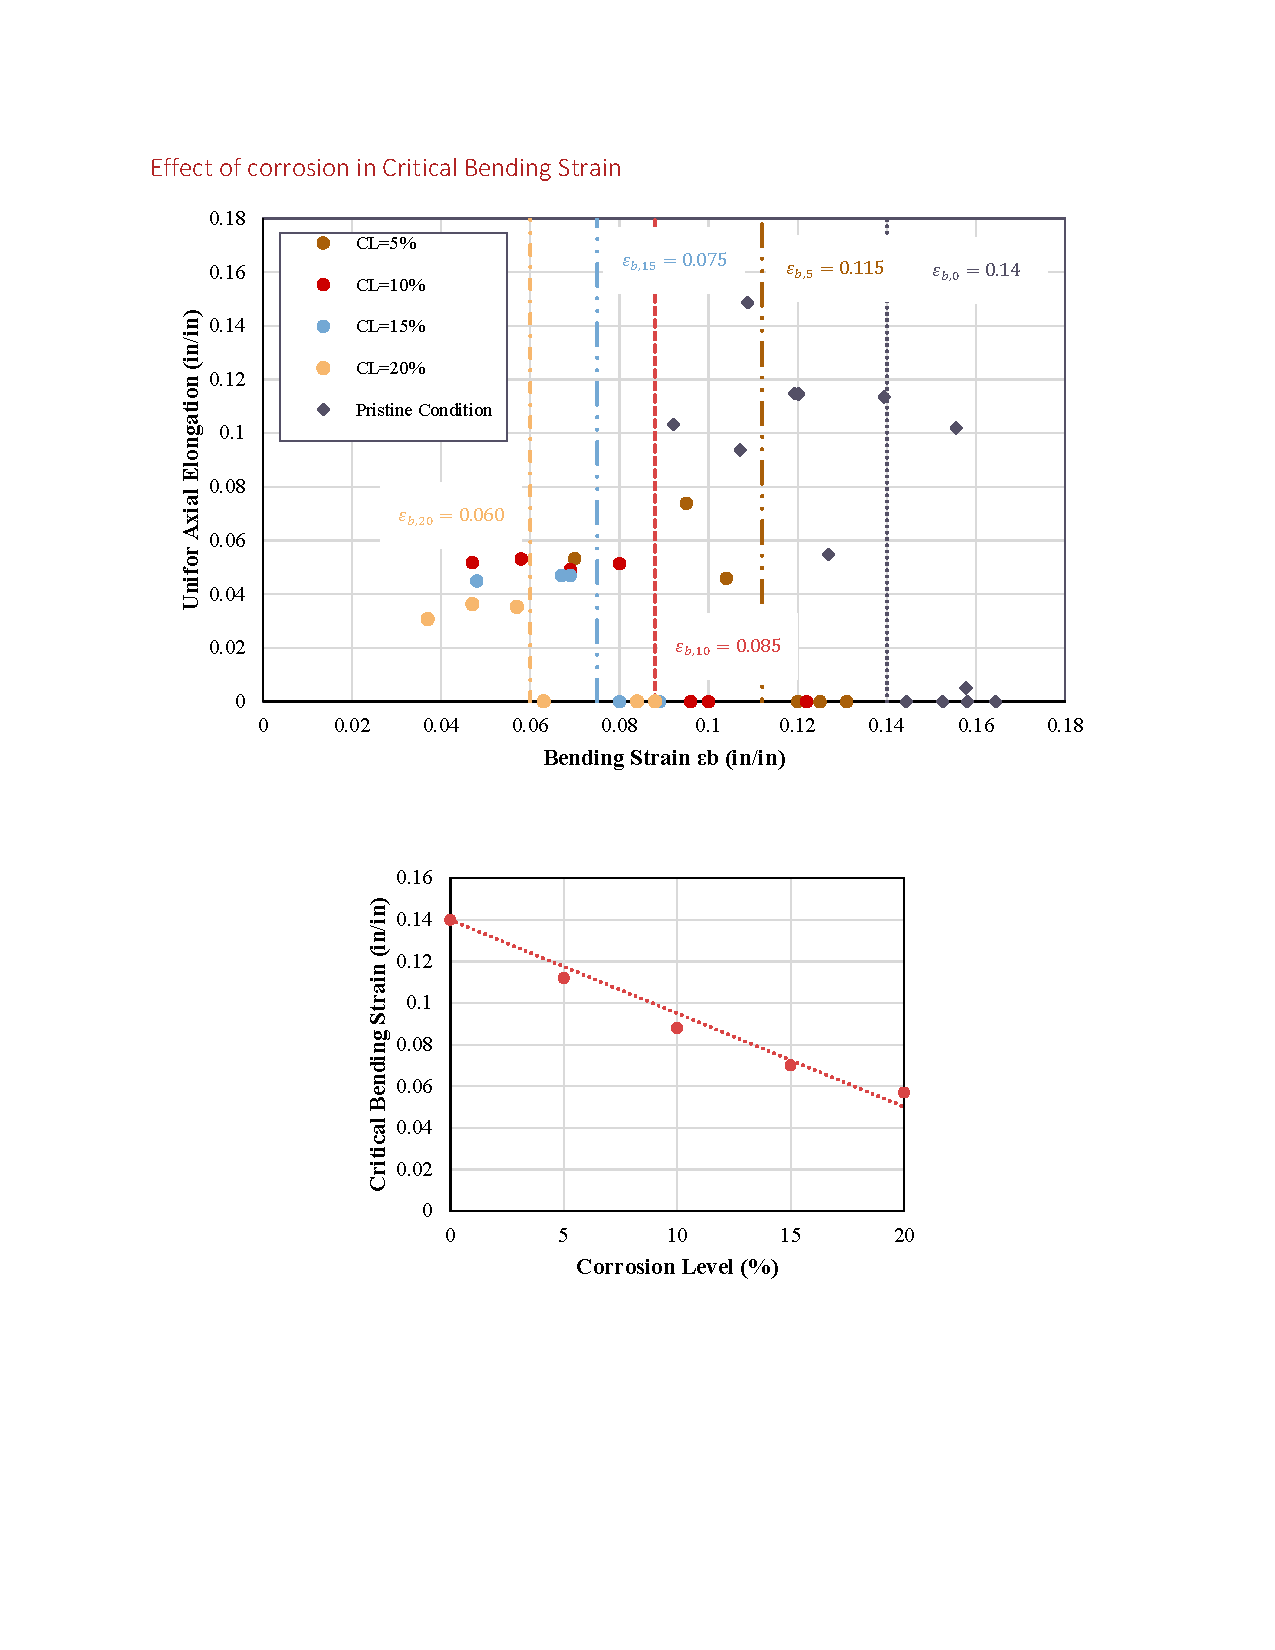
\includegraphics[width=0.7\textwidth]{VAC Thesis 2.0/Chapter-4/figs/BBT_results_.pdf}
	\caption{Bending strain at different corrosion levels}
	\label{fig:BBT_strains}
\end{figure}
\begin{figure}[htbp]
	\centering
	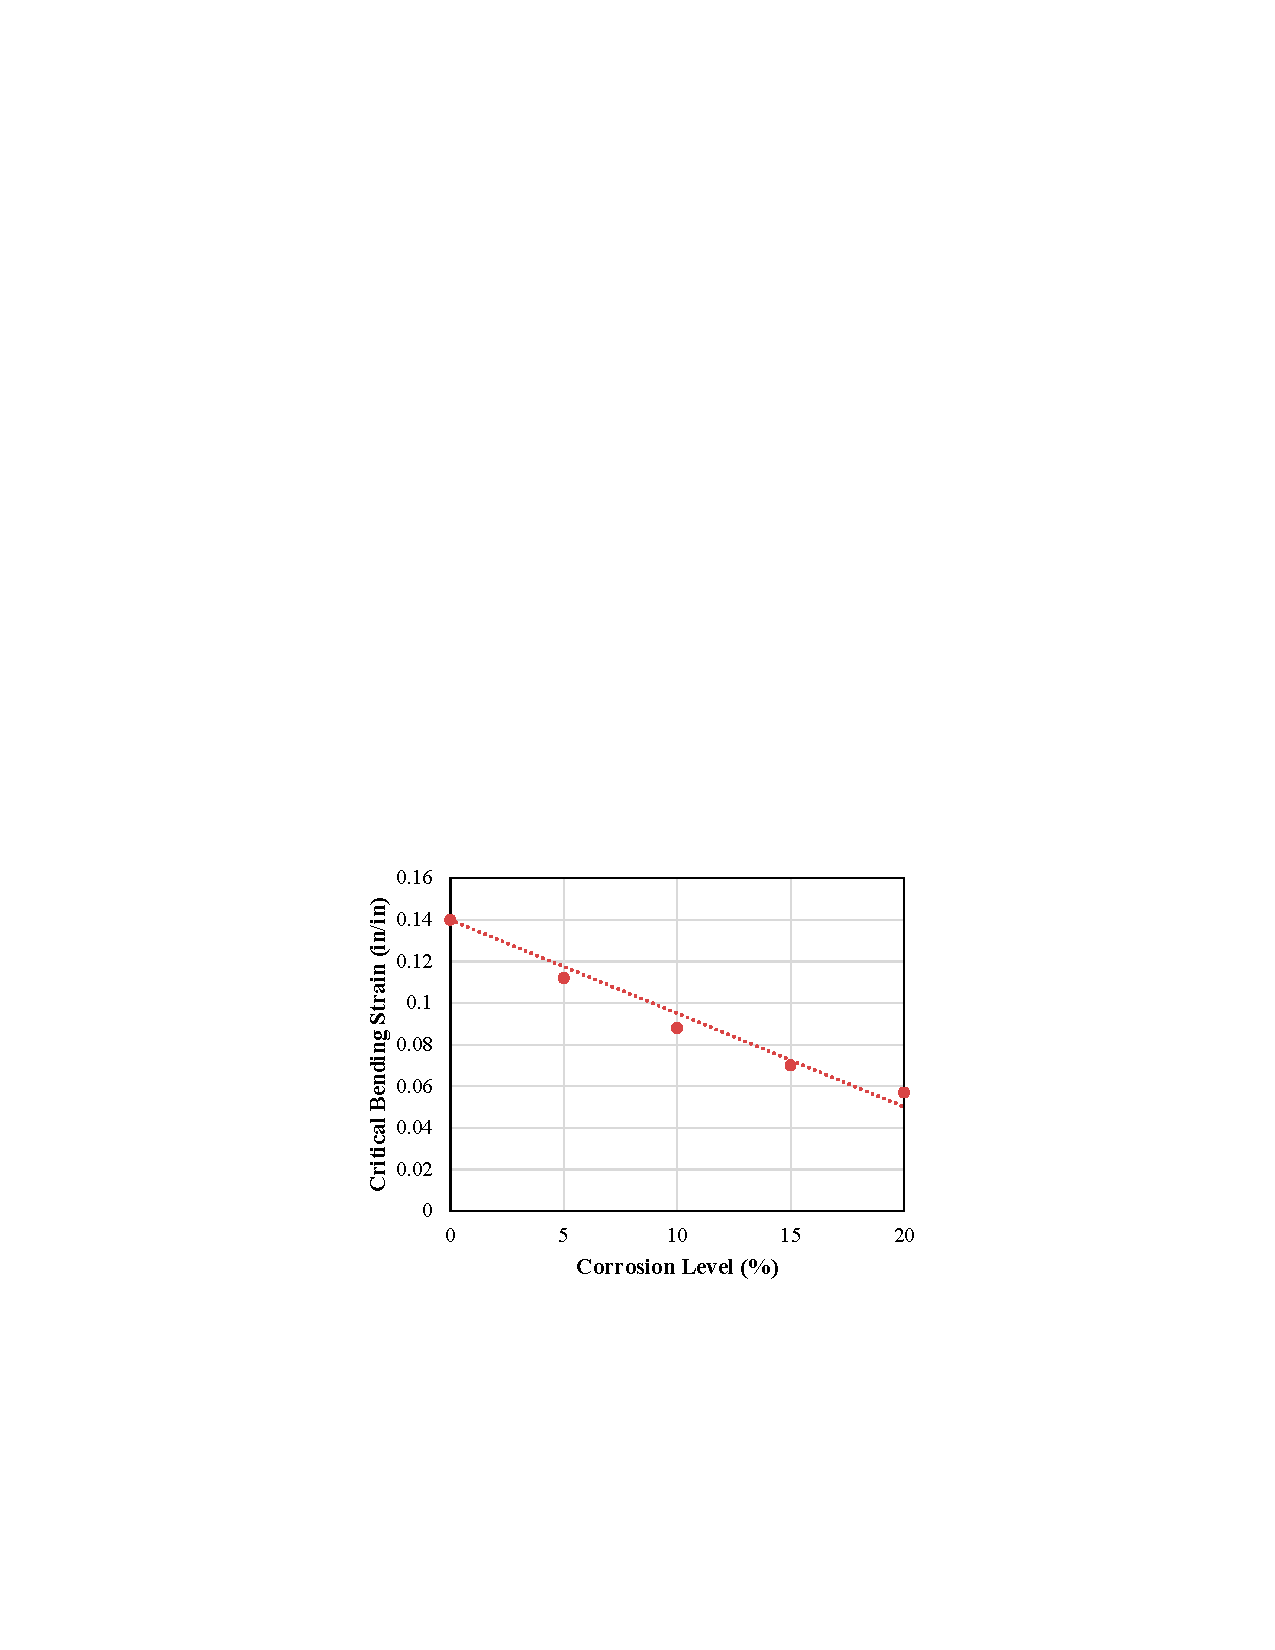
\includegraphics[width=0.7\textwidth]{VAC Thesis 2.0/Chapter-4/figs/BBT_results_summary.pdf}
	\caption{Maximum bending strain as a function of corrosion level}
	\label{fig:eb_vs_CL}
\end{figure}

\subsection{Effect of corrosion at the micro-structural level}

\textbf{Fractography}

\begin{figure}[htbp]
	\centering
	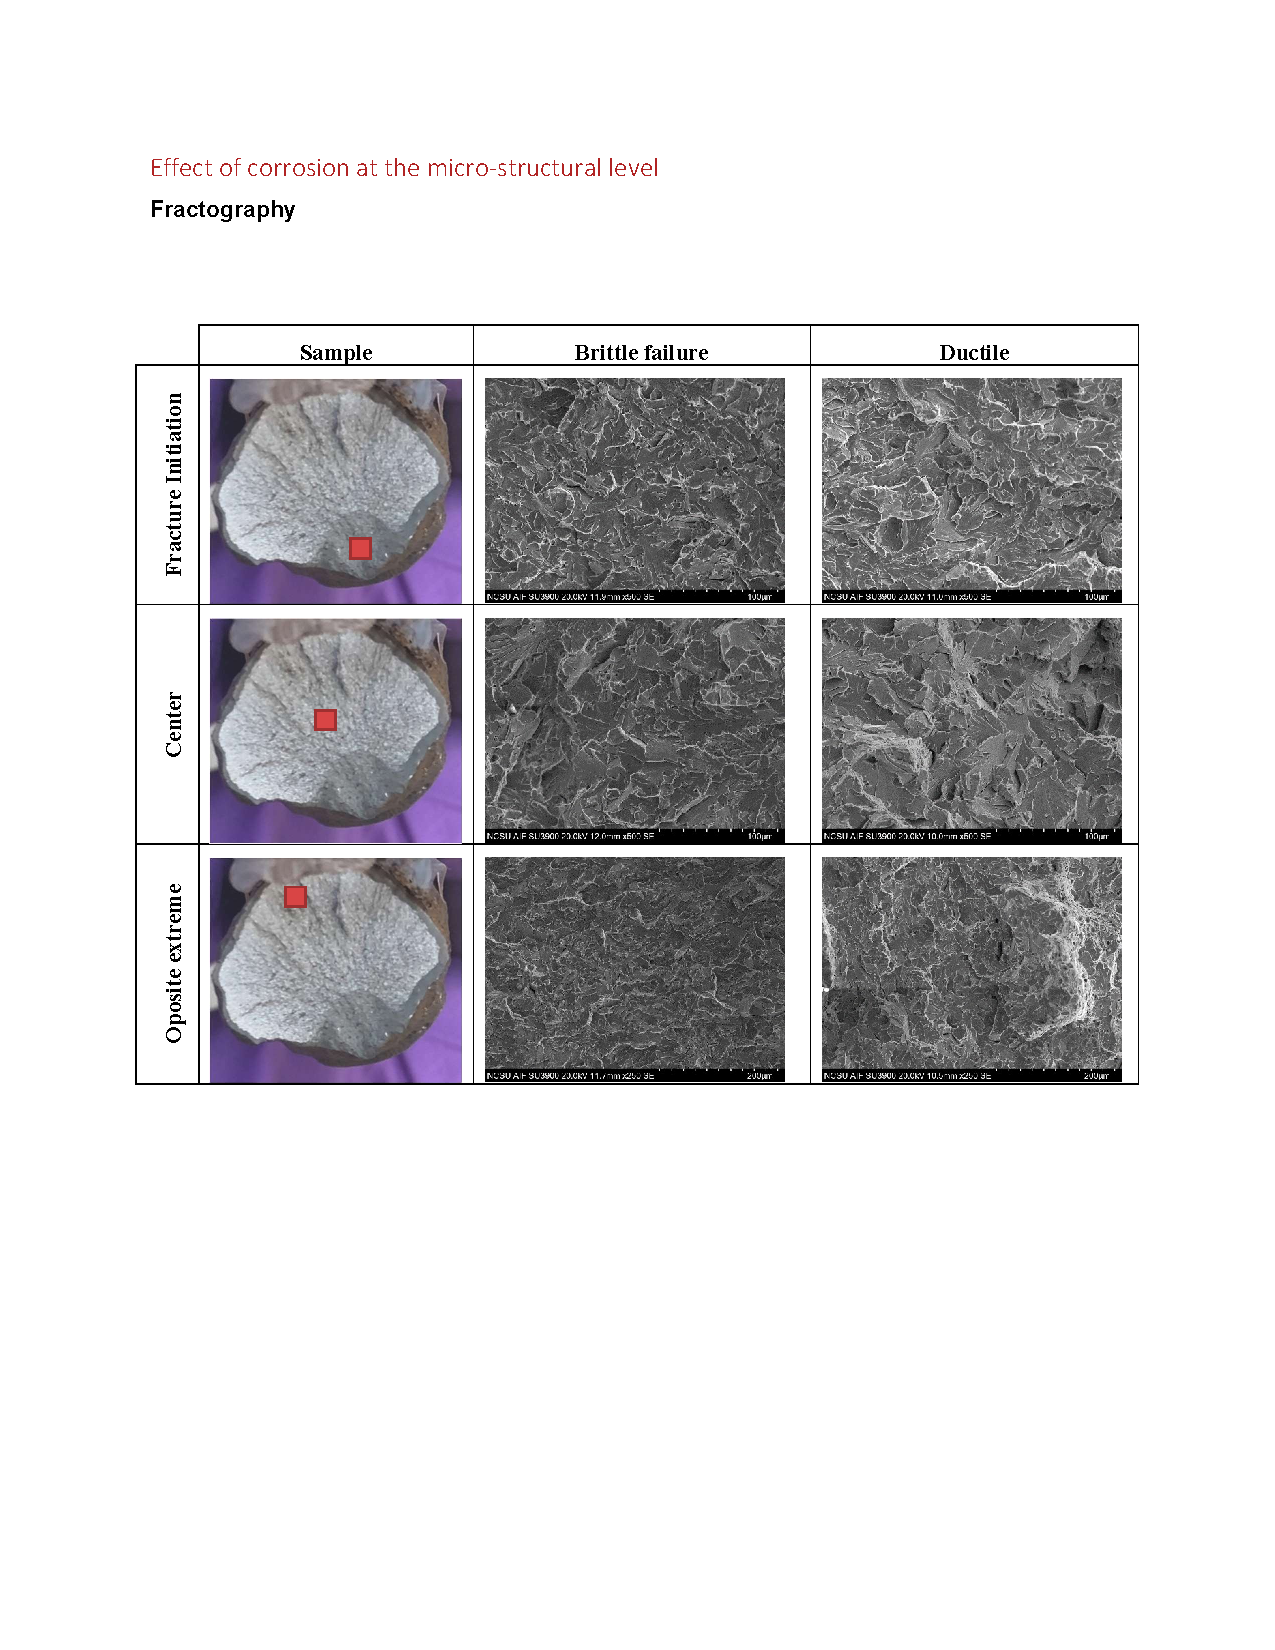
\includegraphics[width=1\textwidth]{VAC Thesis 2.0/Chapter-4/figs/BBT_fractography.pdf}
	\caption{SEM observations for brittle and ductile failure at different positions of the fracture surface}
	\label{fig:FractureSurfaces}
\end{figure}
\begin{figure}[htbp]
	\centering
	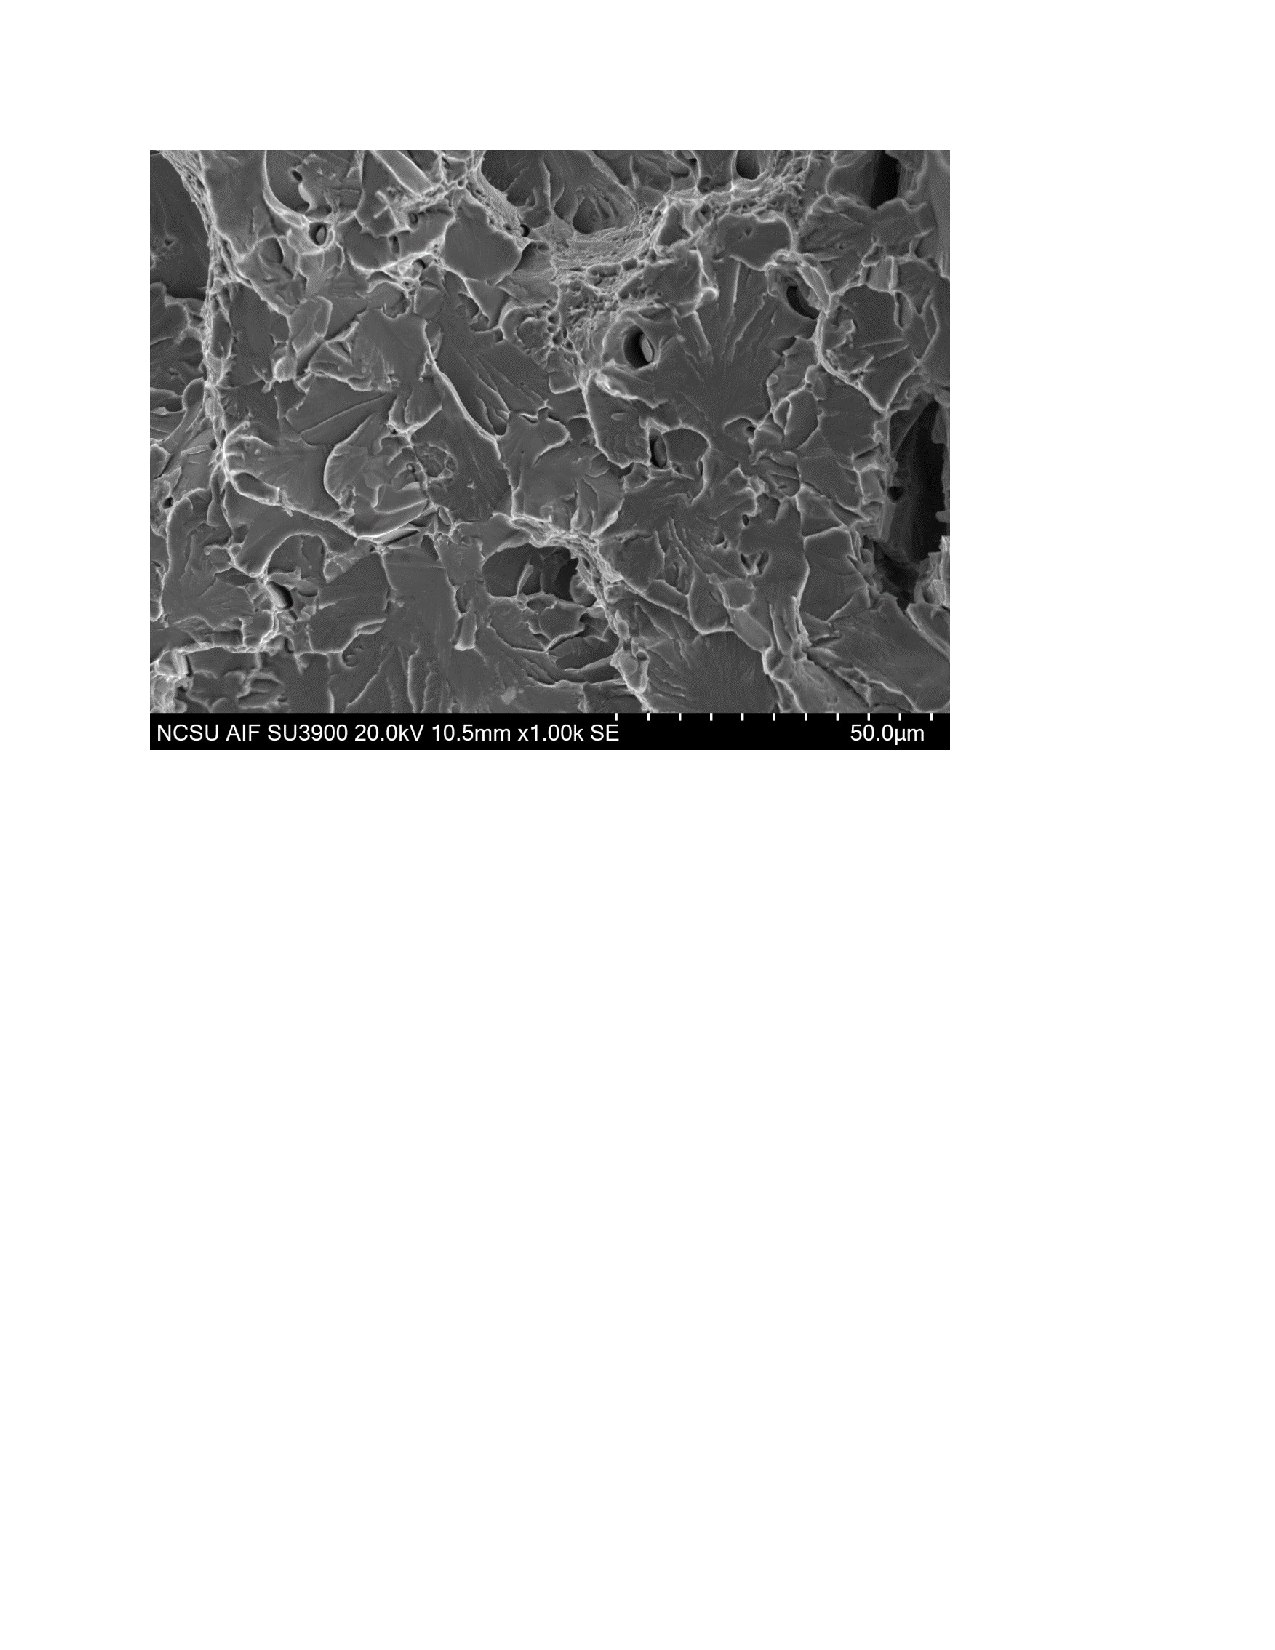
\includegraphics[width=0.7\textwidth]{VAC Thesis 2.0/Chapter-4/figs/BBT_RiverFeatures.pdf}
	\caption{SEM cyclic loading features in fracture surface at 500x magnification}
	\label{fig:RiverFeatures}
\end{figure}

\textbf{Spectrum analysis}
\begin{figure}[htbp]
	\centering
	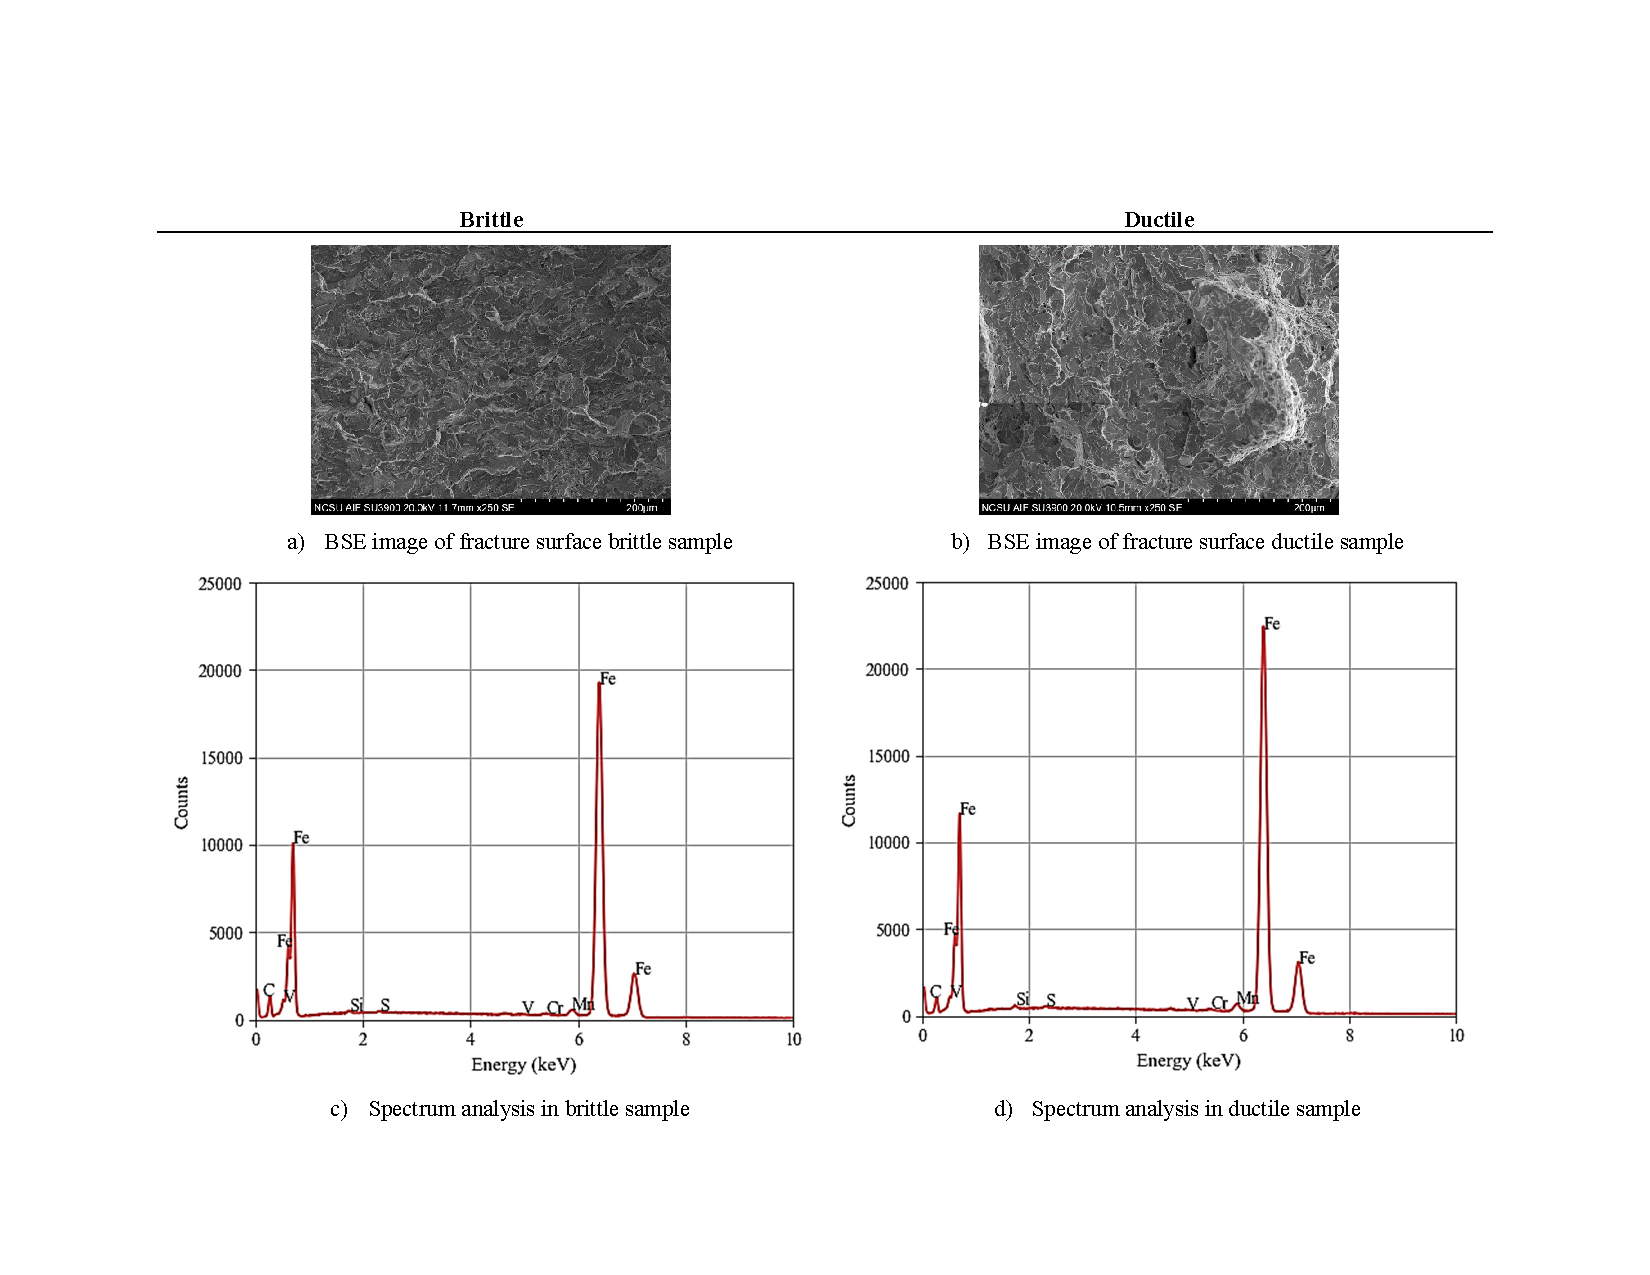
\includegraphics[width=0.9\textwidth]{VAC Thesis 2.0/Chapter-4/figs/BBT_SpectrumAnalysis.pdf}
	\caption{Spectrum analysis of Back Scatter Electrons of fracture surface for brittle and ductile failures}
	\label{fig:SpectrumAnalysis}
\end{figure}
\subsection{Effect of geometry imperfections}